\documentclass[11pt, oneside]{article}
\usepackage[letterpaper, margin=2cm]{geometry}
\usepackage{MATH667}

\begin{document}
\noindent \textbf{\Large{Caleb Logemann \\
MATH667 Hyperbolic Partial Differential Equations \\
Homework 2
}}

%\lstinputlisting[language=MATLAB]{H01_23.m}
\begin{enumerate}
  \item % #1 Done
    Determine the exact solution to Burgers' equation for all $t > 0$, with the
    following initial data sets.
    \begin{enumerate}
      \item[(a)] % Done
        \[
          u(x,0) =
          \begin{cases}
            1 & x < -1 \\
            0 & -1 \le x \le 1 \\
            -1 & x > 1
          \end{cases}
        \]

        Initially there are two discontinuities with $u_l > u_r$.
        Using the Rankine-Hugionot condition for Burgers' equation we see that the
        shock speed for the left discontinuity is $1/2$ and the shock speed
        for the right discontinuity is $-1/2$.
        So the shock locations can be described with the following equations
        \begin{align*}
          x_l(t) &= \frac{1}{2}t - 1 \\
          x_r(t) &= -\frac{1}{2}t + 1
        \end{align*}
        Note that these shocks are moving towards each other.
        They will meet when
        \[
          \frac{1}{2}t - 1 = -\frac{1}{2}t + 1
        \]
        Solving this shows that the shocks meet when $t = 2$ at $x = 0$.
        Now a new shock speed must be determined.
        The average of the left and right states is now $0$, so the shock speed
        is $0$.
        This implies that there is a standing shock wave at $x = 0$, when
        $t > 2$.

        Now the full solution can be expressed as follows
        \[
          u(x, t) =
          \begin{cases}
             1 & t < 2 \text{ and } x < \frac{1}{2}t - 1 \\
             0 & \frac{1}{2}t - 1 < x < -\frac{1}{2}t + 1 \\
            -1 & t < 2 \text{ and } x > -\frac{1}{2}t + 1 \\
             1 & t > 2 \text{ and } x < 0 \\
            -1 & t > 2 \text{ and } x > 0
          \end{cases}
        \]

        The following image is a graphical description of this solution.
        \begin{center}
          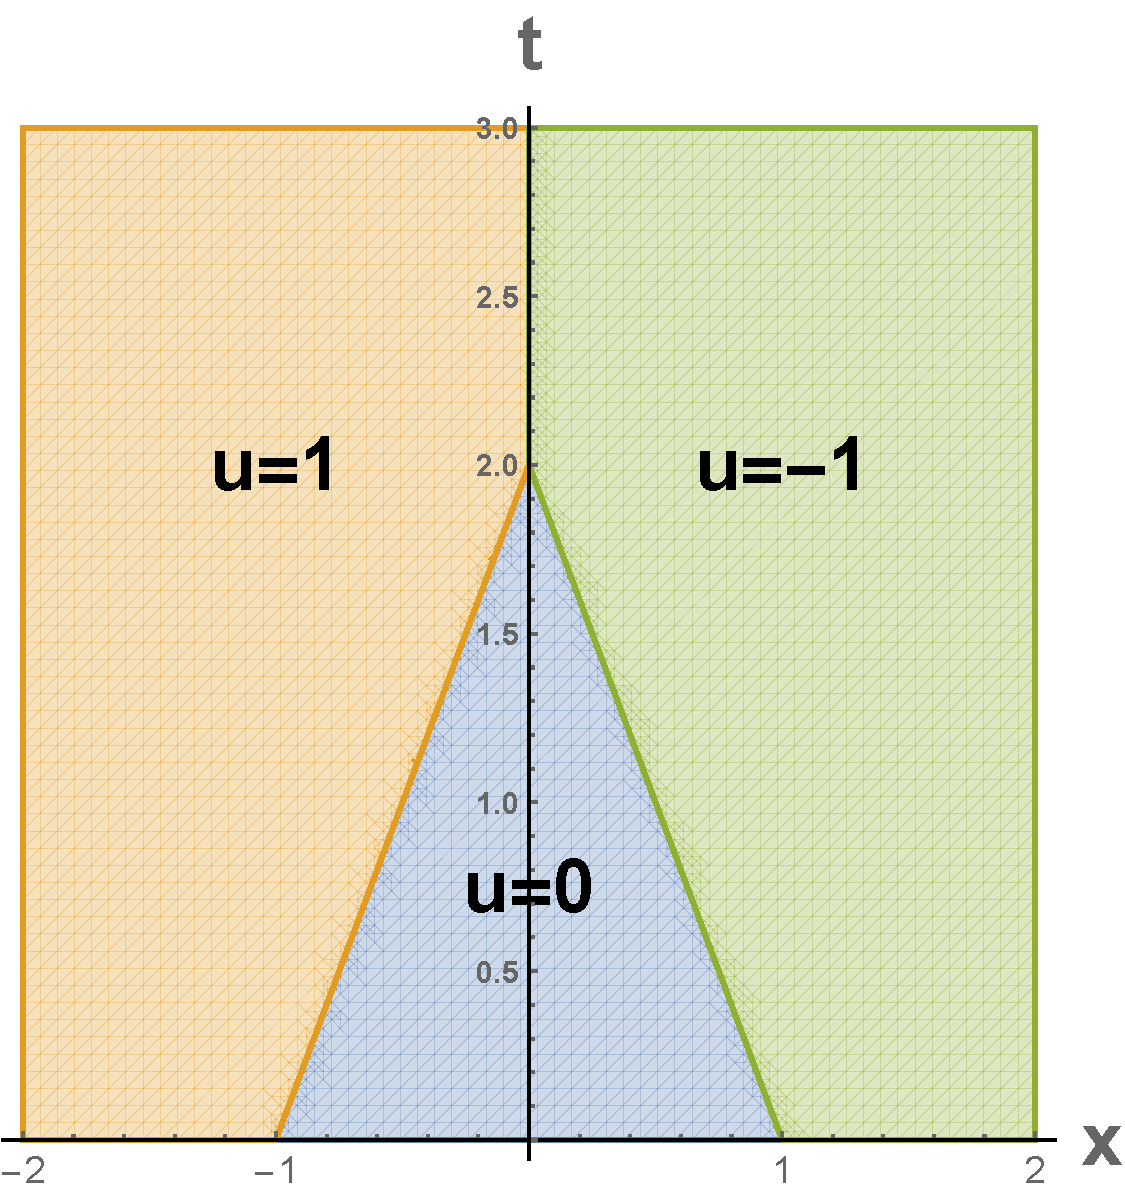
\includegraphics[scale=0.3]{Figures/02_1a.pdf}
        \end{center}

      \item[(b)] % Done
        \[
          u(x,0) =
          \begin{cases}
            -1 & x < -1 \\
            0 & -1 \le x \le 1 \\
            1 & x > 1
          \end{cases}
        \]

        In this case we start with two discontinuities with $u_l < u_r$.
        Both of these discontinuities will result in a rarefaction.
        For the left rarefaction the boundaries of the rarefaction
        will be $x = -1$ and $x = -t - 1$.
        For the right rarefaction the boundaries will be $x = 1$ and $x = t + 1$.
        On a standard rarefaction centered at $x = 0$ for Burgers' equation the
        boundaries are $x = u_r t$ and $x = u_l t$, however these cases need to
        encorporate the shift to $x = \pm 1$.
        The full solution is thus
        \[
          u(x, t) =
          \begin{cases}
            -1 & x < -t - 1 \\
            \frac{x}{t} & -t - 1 < x < -1 \\
            0 & -1 < x < 1 \\
            \frac{x}{t} & 1 < x < t + 1 \\
            1 & x > 1
          \end{cases}
        \]
        \begin{center}
          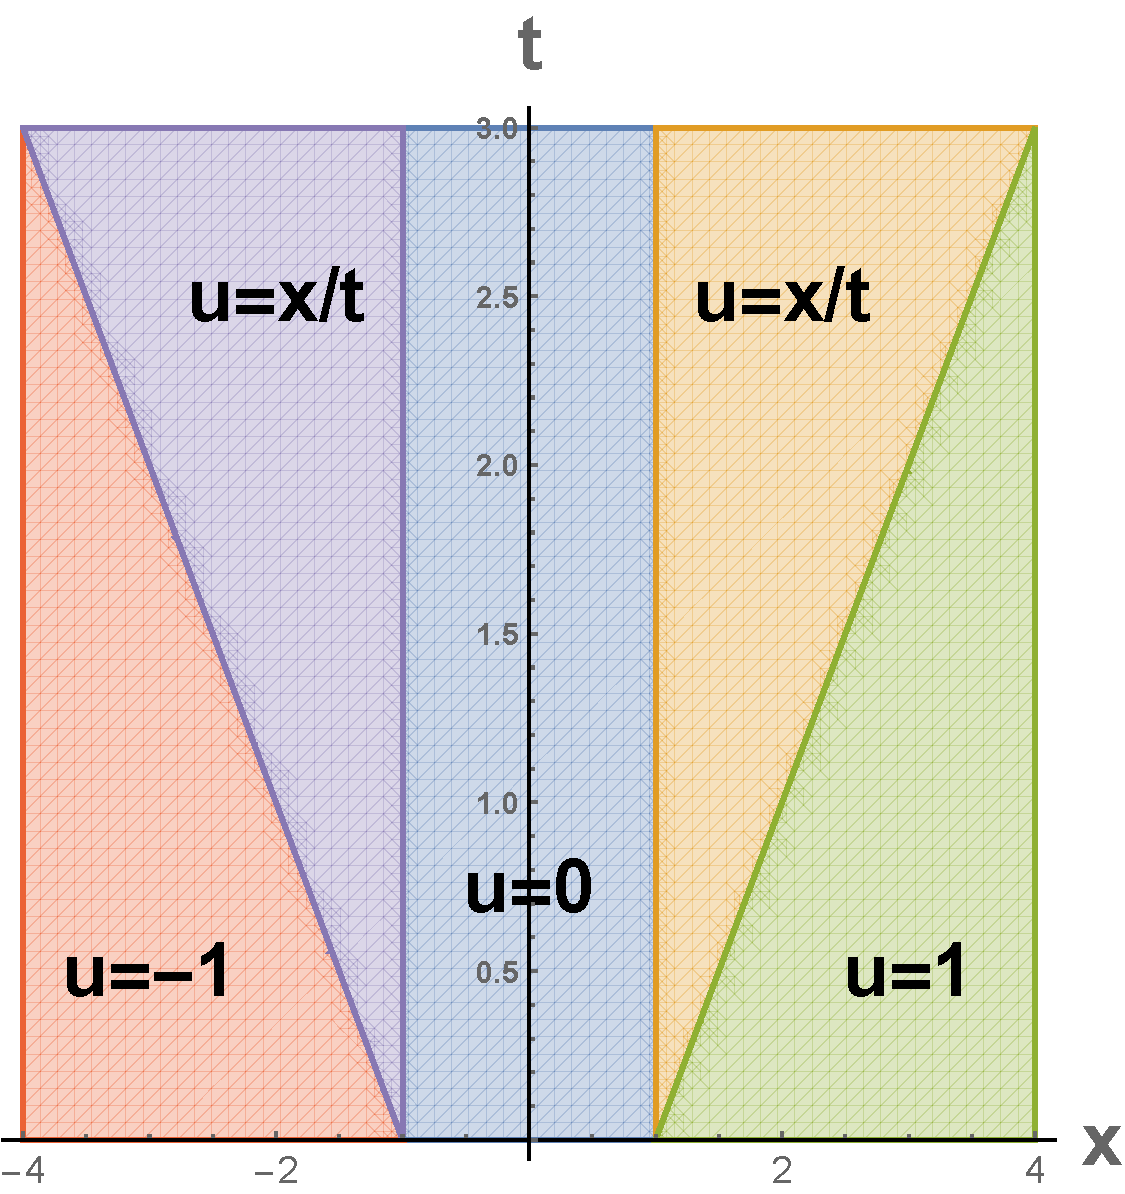
\includegraphics[scale=0.3]{Figures/02_1b.pdf}
        \end{center}

      \item[(c)] % Done
        \[
          u(x,0) =
          \begin{cases}
            12 & x < 0 \\
            8 & 0 \le x <  14 \\
            4 & 14 \le x \le 17 \\
            2 & x \ge 17
          \end{cases}
        \]

        This problem starts with three discontinuities all with $u_l > u_r$.
        The left most shock will propogate with speed $(12 + 8)/2 = 10$, so the
        location of this shock is $x_l(t) = 10t$.
        The middle shock will propogate with speed $(8 + 4)/2 = 6$ from initial
        location $x = 14$.
        Thus the location of this shock in time is $x_m(t) = 6t + 14$.
        The rightmost shock will propogate with speed $(4 + 2)/2 = 3$ starting
        from $x = 17$, so the location of this shock will be $x_r(t) = 3t + 17$.

        Now these shocks will at some point in time meet.
        To find this time we must solve $x_l(t) = x_m(t)$ and $x_m(t) = x_r(t)$.
        \begin{align*}
          10t &= 6t + 14 \\
          4t &= 14 \\
          t &= \frac{7}{2}
        \end{align*}
        and
        \begin{align*}
          6t + 14 &= 3t + 17 \\
          3t &= 3 \\
          t &= 1
        \end{align*}
        This shows that the middle and rightmost shocks will meet first at
        $(x, t) = (20, 1)$.
        When the do meet the new shock speed will be $(8 + 2)/2 = 5$ and the
        location of this shock will be $x_{mr}(t) = 5(t - 1) + 20 = 5t + 15$.

        Now the last two shocks will meet when $x_l(t) = x_{mr}(t)$.
        \begin{align*}
          10t &= 5(t - 1) + 20 \\
          5t &= 15 \\
          t & = 3
        \end{align*}
        These two shocks will meet at $(x, t) = (30, 3)$.
        They will merge into a single final shock with speed $(12 + 2)/2 = 7$
        and location $x_{lmr}(t) = 7(t - 3) + 30 = 7t + 9$.

        The full solution can now be expressed as
        \[
          u(x, t) =
          \begin{cases}
            12 & \p{t < 3 \text{ and } x < 10t} \text{ or } \p{t > 3 \text{ and } x < 7t + 9} \\
            8 & \p{t < 1 \text{ and } 10t < x < 6t + 14} \text{ or } \p{1 < t < 3 \text{ and } 10t < x < 5t + 15}  \\
            4 & 6t + 14 < x < 3t + 17 \\
            2 & \p{t < 1 \text{ and } 3t + 17 < x} \text{ or } \p{ 1 < t < 3 \text{ and } x > 5t + 15} \text { or } \p{t > 3 \text{ and } x > 7t + 9}
          \end{cases}
        \]

        \begin{center}
          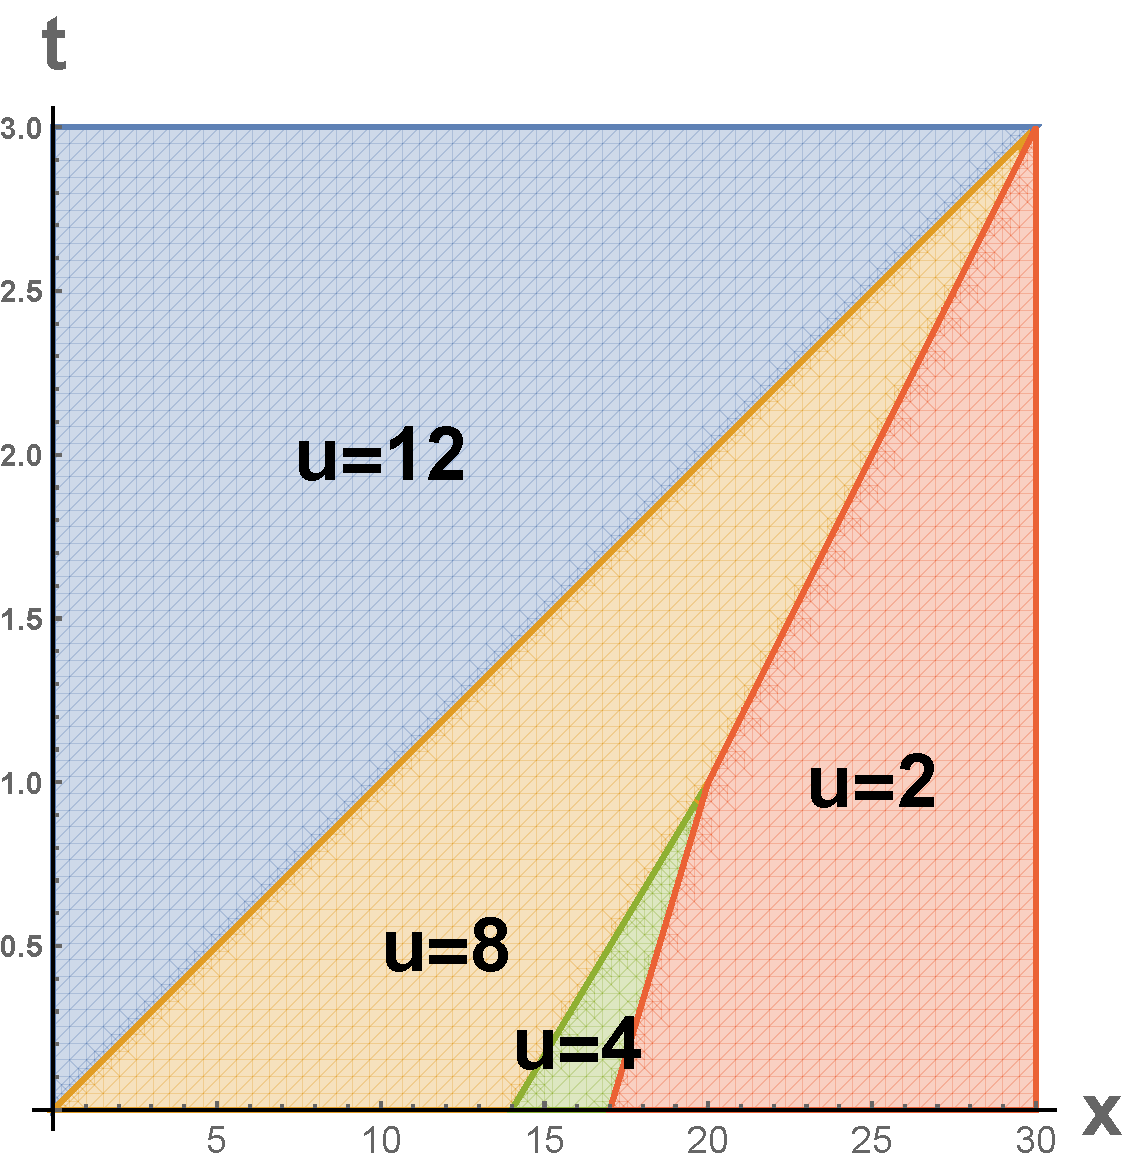
\includegraphics[scale=0.3]{Figures/02_1c.pdf}
        \end{center}

      \item[(d)] % Done
        \[
          u(x,0) =
          \begin{cases}
            0 & x < 0 \\
            2 & 0 \le x \le 1 \\
            0 & x > 1
          \end{cases}
        \]

        This problem starts with two discontinuities one with $u_l < u_r$ and
        one with $u_l > u_r$.
        The left discontinuity will result in a rarefaction with endpoints
        $x = 0$ and $x = 2t$.
        The right discontinuity will result in a shock propogating at speed
        $(2 + 0)/2 = 1$, with location $x(t) = t + 1$.
        When $2t = t + 1$ the rarefaction and shock will meet, that is at
        $t = 1$
        At this time the left hand side of the shock will now be $x/t$, and
        this will cause the shock speed to decrease over time.
        However we can describe the solution for $t < 1$.
        \[
          u(x, t) =
          \begin{cases}
            0 & x < 0 \\
            \frac{x}{t} & 0 < x < 2t \\
            2 & 2t < x < t + 1 \\
            0 & t + 1 < x
          \end{cases}
        \]

        \begin{center}
          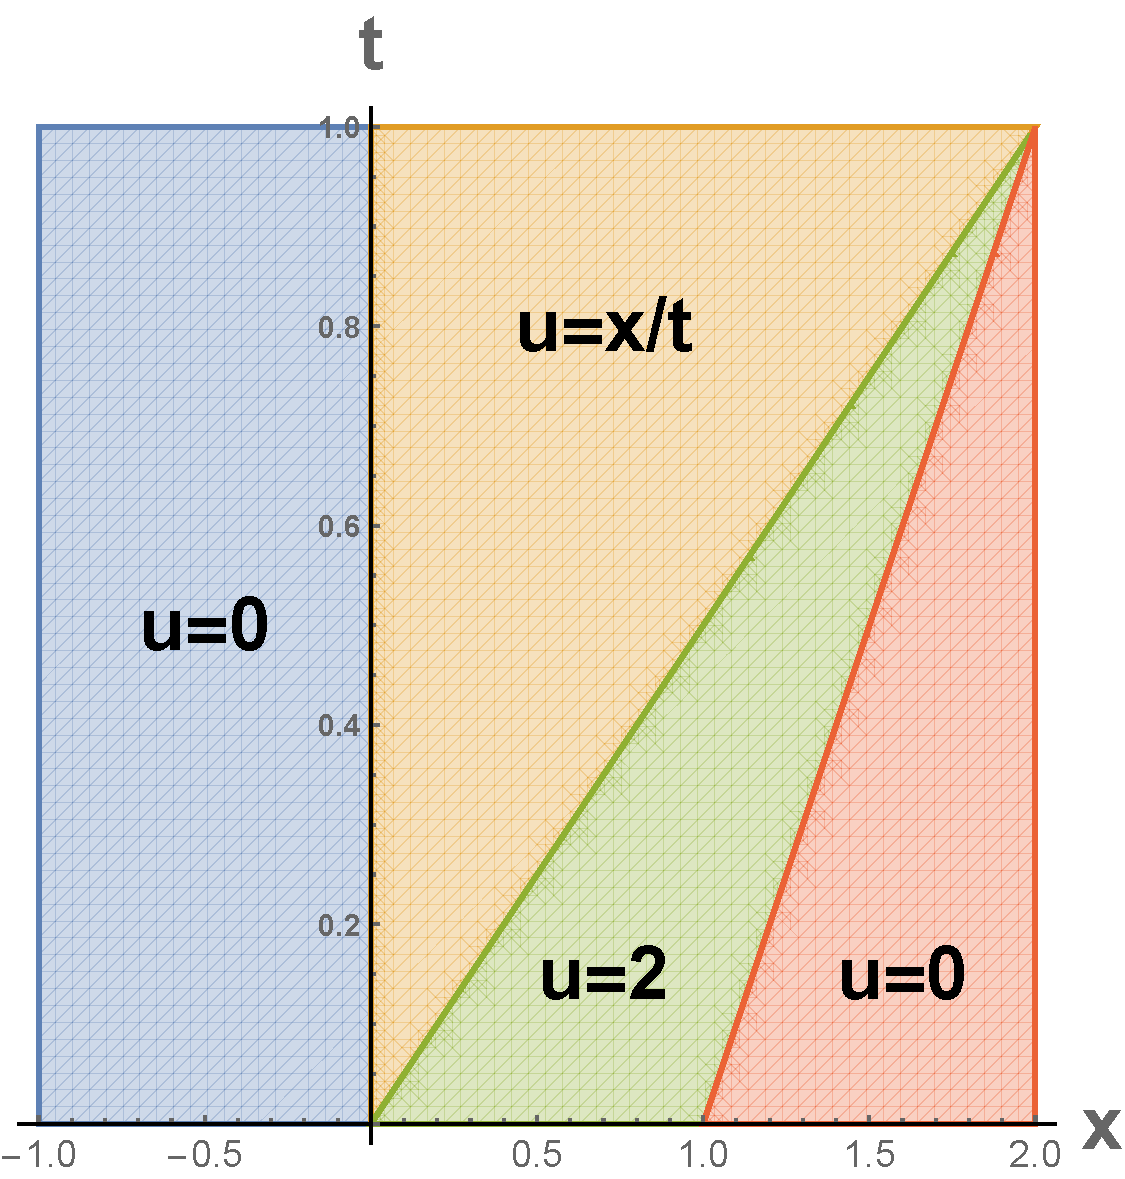
\includegraphics[scale=0.3]{Figures/02_1d.pdf}
        \end{center}
    \end{enumerate}

  \item % #2 Done
    Consider the simple wave equation $u_t + u_x = 0$, derive the local
    truncation error of the Lax-Friedrichs and Lax-Wendroff schemes:
    \[
      \text{Lax-Friedrichs:} u_j^{n+1} = u_j^n
      - \Delta t \frac{u_{j+1}^n - u_{j-1}^n}{2\Delta x}
      + \frac{\Delta x^2}{2} \frac{u_{j+1}^n - 2u_j^n + u_{j-1}^n}{\Delta x^2}
    \]
    \[
      \text{Lax-Wendroff:} u_j^{n+1} = u_j^n
      - \Delta t \frac{u_{j+1}^n - u_{j-1}^n}{2\Delta x}
      + \frac{\Delta t^2}{2} \frac{u_{j+1}^n - 2u_j^n + u_{j-1}^n}{\Delta x^2}
    \]

    First I will consider the Lax-Friedrichs method.
    The truncation error can be expressed as
    \[
      \tau_j^n = \frac{u_j^{n+1} - u_j^n}{\Delta t}
      + \frac{u_{j+1}^n - u_{j-1}^n}{2\Delta x}
      - \frac{\Delta x^2}{2 \Delta t} \frac{u_{j+1}^n - 2u_j^n + u_{j-1}^n}{\Delta x^2}
    \]

    Next I will substitue in the exact solution to the PDE, $u(x, t)$,
    and I will shorthand $u = u(x_j, t^n)$.
    I will simplify using the following Taylor expansions.
    \begin{align*}
      u_j^n &= u(x_j, t^n) = u \\
      u_j^{n+1} &= u(x_j, t^n + \Delta t) = u + \Delta t u_t + O(\Delta t^2) \\
      u_{j+1}^n &= u(x_j + \Delta x, t^n) = u + \Delta x u_x + \frac{1}{2}\Delta x^2 u_{xx} + O(\Delta x^3) \\
      u_{j-1}^n &= u(x_j - \Delta x, t^n) = u - \Delta x u_x + \frac{1}{2}\Delta x^2 u_{xx} + O(\Delta x^3)
    \end{align*}

    Now I will simplify the three main terms in the truncation error expression.
    \begin{align*}
      \frac{u_j^{n+1} - u_j^n}{\Delta t} &= \frac{u + \Delta t u_t + O(\Delta t^2) - u}{\Delta t} \\
      &= u_t + O(\Delta t)
    \end{align*}
    \begin{align*}
      \frac{u_{j+1}^n - u_{j-1}^n}{2\Delta x} &= \frac{2\Delta x u_x + O(\Delta x^3)}{2\Delta x} \\
      &= u_x + O(\Delta x^2) \\
    \end{align*}
    \begin{align*}
      -\frac{\Delta x^2}{2 \Delta t} \frac{u_{j+1}^n - 2u_j^n + u_{j-1}^n}{\Delta x^2} &= -\frac{\Delta x^2}{2 \Delta t} \frac{\Delta x^2 u_{xx} + O(\Delta x^3)}{\Delta x^2} \\
      &= -\frac{\Delta x^2}{2 \Delta t} \p{u_{xx} + O(\Delta x)} \\
    \end{align*}

    Now the truncation error can be expressed as
    \[
      \tau_j^n = u_t + O(\Delta t) + u_x + O(\Delta x^2) - \frac{\Delta x^2}{2 \Delta t} \p{u_{xx} + O(\Delta x)}
    \]
    Since $u$ is a solution to the PDE, $u_t + u_x = 0$
    Now the truncation error is
    \[
      \tau_j^n =  O(\Delta t + \Delta x^2) - \frac{\Delta x^2}{2 \Delta t} \p{u_{xx} + O(\Delta x)}
    \]

    Next I will do the truncation error for the Lax-Wendroff method.
    \[
      \tau_j^n = \frac{u_j^{n+1} - u_j^n}{\Delta t}
      + \frac{u_{j+1}^n - u_{j-1}^n}{2\Delta x}
      - \frac{\Delta t}{2} \frac{u_{j+1}^n - 2u_j^n + u_{j-1}^n}{\Delta x^2}
    \]
    I will use the same notation and Taylor series as earlier.
    Only the third term is different
    \begin{align*}
      -\frac{\Delta t}{2} \frac{u_{j+1}^n - 2u_j^n + u_{j-1}^n}{\Delta x^2} &= -\frac{\Delta t}{2} \frac{\Delta x^2 u_{xx} + O(\Delta x^3)}{\Delta x^2} \\
      &= -\frac{\Delta t}{2} \p{u_{xx} + O(\Delta x)}
    \end{align*}

    Now the local truncation error is
    \[
      \tau_j^n = u_t + O(\Delta t) + u_x + O(\Delta x^2) -\frac{\Delta t}{2} \p{u_{xx} + O(\Delta x)}
    \]
    Again since $u$ is a solution to the PDE, $u_t + u_x = 0$
    Now the truncation error is
    \[
      \tau_j^n = O(\Delta t + \Delta x^2) -\frac{\Delta t}{2} \p{u_{xx} + O(\Delta x)}
    \]

  \item % #3 Done
    The following function implements the Lax-Friedrichs method.
    \lstinputlisting[language=MATLAB]{laxFriedrichs.m}
    The following function implements the Lax-Wendroff method.
    \lstinputlisting[language=MATLAB]{laxWendroff.m}

    The following script now uses the previous two methods along with the
    upwind method from homework 1 to compute a solution to the advection
    equation.
    \lstinputlisting[language=MATLAB]{H02.m}
    The following two images are produced.
    Note that the Lax-Wendroff method has the least amount of decay but it does
    have oscillations around the discontinuites.
    The upwind and Lax-Friedrichs method decay the solution more, with the
    Upwind method being slightly better.
    \begin{center}
      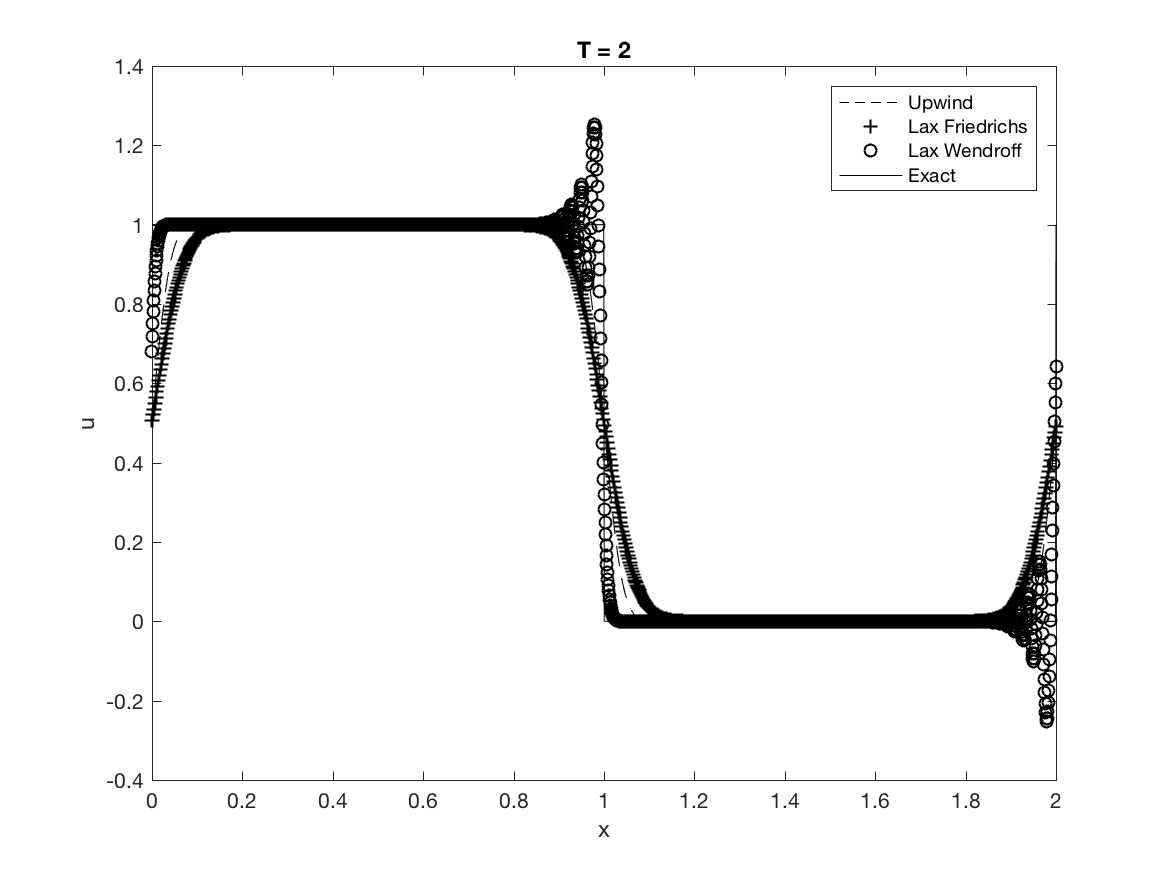
\includegraphics[scale=0.5]{Figures/02_01.png}
      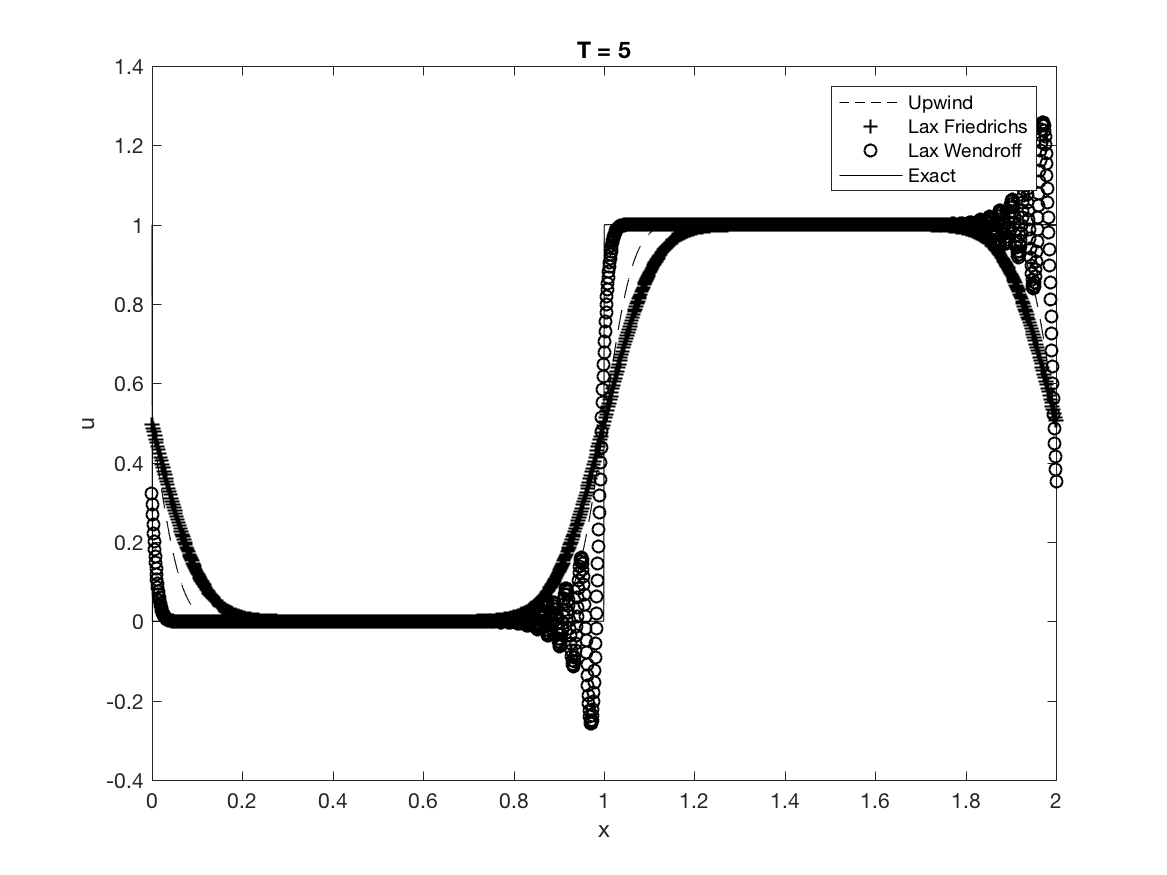
\includegraphics[scale=0.5]{Figures/02_02.png}
    \end{center}

\end{enumerate}
\end{document}
